% =============================================================================
% Definicao do mercado (projeto Riachuelo, PRO3474). Item A do roteiro.
%
% Adaptado do documento "1 PANORAMA DO MERCADO DE VAREJO DE MODA E PRINCIPAIS
% TENDENCIAS" (docx da equipe), reescrito no padrao do relatorio. Referencias
% em bibliografia.bib (chaves *2023*, *2024*, *2025*, *2026*). A Figura de
% receita e a imagem original do documento.
% =============================================================================

\section{DEFINIÇÃO DO MERCADO}
\label{sec:mercado}
\nocite{startse2023autoatendimento} % consta nas referencias do documento original

\subsection{Panorama do varejo de moda}
\label{subsec:panorama}

O varejo de moda no Brasil é um mercado de grande escala e estruturalmente pulverizado. Segundo estimativa da Associação Brasileira do Varejo Têxtil (ABVTEX), o setor têxtil brasileiro, que engloba vestuário, calçados e artigos de cama, mesa e banho, faturou R\$ 427,1 bilhões em 2025. No mesmo ano, as 11 maiores empresas de moda de capital aberto do país somaram receita líquida de R\$ 60,35 bilhões, o equivalente a apenas 15\% desse faturamento \cite{gbljeans2026maiores}. O setor é, portanto, fragmentado no conjunto, embora parte relevante da receita se concentre em poucas redes de grande porte.

O peso dessas redes aparece também no desempenho recente das varejistas listadas em bolsa. No segundo trimestre de 2025, três das quatro maiores varejistas de moda do país registraram crescimento de receita líquida superior a 10\% em relação ao ano anterior: a Renner cresceu 18,5\%, a Riachuelo 13,9\% e a C\&A 12,4\%, enquanto a Azzas 2154 teve alta de 4,8\% \cite{timesbrasil2025varejistas}. O crescimento se manteve ao longo de 2025 e 2026, e no segundo trimestre de 2026 Renner, C\&A e Riachuelo somaram R\$ 8,9 bilhões em receita líquida consolidada, com a Riachuelo apresentando o maior crescimento proporcional entre as três, de 8,9\% na receita líquida de vestuário \cite{gbljeans2026trimestre}.

\subsection{Tendências globais do varejo de moda}
\label{subsec:tendencias}

O relatório \textit{Fashion Retail Outlook 2026}, da Strategy\&, consultoria de estratégia da PwC, aponta quatro tendências para o varejo de moda global \cite{strategyand2026outlook}. A primeira é a rastreabilidade e a transparência de produto, impulsionada pela exigência de Passaportes Digitais de Produto pela União Europeia a partir de 2027, que torna a origem e a composição das peças um diferencial de compra. A segunda é o comércio agêntico, isto é, a compra de moda mediada por assistentes de inteligência artificial, com parcela relevante dos consumidores pesquisados disposta a comprar diretamente por meio desses assistentes. A terceira é o reforço da resiliência da cadeia de suprimentos por meio de \textit{nearshoring} e microfabricação local, em resposta a tensões geopolíticas e tarifárias. A quarta é o que a consultoria chama de equação de ``valor inteligente'', em que a combinação entre preço, relevância de tendência e qualidade passa a decidir a compra no lugar da competição baseada apenas em preço.

Essa última tendência tem relação direta com o projeto. Segundo o relatório, o peso de cada fator varia conforme o posicionamento do varejista: no \textit{mass market}, preço e relevância de tendência dominam, e qualidade e durabilidade ficam em segundo plano; no premium e no luxo, predominam relevância de tendência e qualidade, e o consumidor é menos sensível ao preço. Essa mesma lógica de posicionamento ajuda a explicar por que o investimento em velocidade de checkout tende a pesar mais no \textit{mass market} e no \textit{fast fashion}, segmentos de alto volume de transações e menor tíquete médio em que a eficiência operacional da loja física faz parte da proposta de valor, do que no premium e no luxo, em que a jornada de compra assistida ainda é vista como parte da experiência.

\subsection{Critérios de segmentação}
\label{subsec:criterios_segmentacao}

Como a solução será vendida a varejistas, em modelo B2B, a equipe considerou quatro critérios para delimitar seu mercado potencial:

\begin{enumerate}[label=\alph*)]
    \item adoção de tecnologia de self-checkout, ou seja, se o varejista já opera terminais de autoatendimento em escala, está em fase de piloto ou ainda não adotou a tecnologia. Esse foi o critério mais determinante, porque a fricção causada pela etiqueta antifurto ganha relevancia apenas em operações que já buscam eliminar etapas manuais do checkout;
    \item porte e escala de operação, medidos por receita líquida, número de lojas e volume diário de transações, que determinam tanto o potencial de receita da venda quanto a complexidade de uma implantação;
    \item posicionamento de marca, \textit{mass market} e \textit{fast fashion} ou premium e luxo, já que a redução de fila é mais relevante para operações de alto volume e menor tíquete médio (Seção~\ref{subsec:tendencias});
    \item categoria de produto (vestuário geral, calçados ou artigos esportivos), pois a maturidade de adoção de RFID e de controles antifurto difere entre elas. No segmento de artigos esportivos, por exemplo, as perdas não identificadas caíram 63,2\% após a adoção de RFID, segundo a 9ª Pesquisa Abrappe de Prevenção de Perdas no Varejo Brasileiro \cite{cartacapital2026perdas}.
\end{enumerate}

\subsection{Segmento-alvo}
\label{subsec:segmento_alvo}

Com base nesses critérios, a equipe definiu como segmento-alvo as redes de moda \textit{mass market} e \textit{fast fashion} que já utilizam, em qualquer estágio de maturidade, tecnologia de self-checkout no Brasil. Esse recorte tem a aderência mais direta ao problema do projeto, porque a remoção manual da etiqueta antifurto rígida só se torna um ponto de atrito relevante, e portanto uma oportunidade comercial, em operações que já investiram em eliminar outras etapas manuais do checkout.

Três grandes redes compõem o núcleo desse segmento, cada uma em um estágio distinto. A Renner é a mais madura: começou a instalar autoatendimento com identificação por radiofrequência em 2019, foi pioneira nessa abordagem no varejo de moda brasileiro e, ao final de 2023, contava com 742 terminais em 213 lojas (52\% da rede), responsáveis por cerca de 38\% dos pagamentos nas lojas em que estão instalados \cite{fashionnetwork2024renner,consumidormoderno2025renner}. Nesses terminais, a tecnologia RFID permite ler todos os itens da compra ao mesmo tempo e desativar o alarme antifurto no momento do pagamento. A Renner já resolveu, assim, a integração entre RFID e antifurto que a Riachuelo ainda não possui, o que a torna ao mesmo tempo referência de \textit{benchmark} e concorrente indireta da solução.

A C\&A ocupa uma posição intermediária. A rede já testa terminais de self-checkout com leitura de código de barras, mas o cliente ainda precisa retirar a etiqueta antifurto manualmente, na lateral do próprio equipamento. A Riachuelo, por sua vez, está em fase de piloto: a primeira loja com self-checkout em todos os caixas foi inaugurada em abril de 2026, no formato de loja conceito do ParkShopping Barigui, em Curitiba, e a rede prevê expandir o formato para mais 15 a 20 lojas ainda em 2026. Essa janela, em que o formato ainda está sendo padronizado para a expansão, concentra a maior oportunidade comercial do projeto.

O gradiente de maturidade dentro do segmento reforça a escolha. A Renner comprova a viabilidade técnica e comercial de integrar leitura automática e antifurto no self-checkout, enquanto os demais integrantes do segmento, a começar pela Riachuelo, ainda não fizeram essa integração.

\subsection{Tamanho do mercado}
\label{subsec:tamanho_mercado}

A estimativa de tamanho de mercado foi construída em três camadas, mercado total endereçável (TAM), mercado endereçável do segmento (SAM) e mercado obtível no curto prazo (SOM), combinando dados do mercado global de tecnologia com dados financeiros dos principais varejistas de moda do Brasil. Os valores de cada camada estão resumidos na Tabela~\ref{tab:tam_sam_som}.

Para o TAM, a equipe considerou duas leituras complementares. Do ponto de vista tecnológico, o mercado global de RFID aplicado ao varejo, que inclui a função antifurto entre suas aplicações, foi estimado em US\$ 15,97 bilhões em 2026, com projeção de US\$ 34,46 bilhões até 2035 e crescimento composto de 8,92\% ao ano \cite{businessresearch2026rfid}. Do ponto de vista do mercado-cliente, o varejo têxtil brasileiro como um todo, com faturamento de R\$ 427,1 bilhões em 2025 \cite{gbljeans2026maiores}, representa o universo de potenciais compradores de tecnologia de checkout e antifurto no país, independentemente de segmento ou porte.

O SAM restringe a análise ao segmento-alvo. Renner, Riachuelo e C\&A somaram R\$ 8,9 bilhões em receita líquida consolidada no segundo trimestre de 2026, dos quais R\$ 6,98 bilhões corresponderam à receita líquida de vestuário das três companhias entre abril e junho \cite{gbljeans2026trimestre}, cuja distribuição entre as redes está na Figura~\ref{fig:receita_vestuario}. Em vendas brutas anuais, métrica mais ampla usada no ranking Top 300 do Varejo Brasileiro, do Instituto Retail Think Tank Brasil, a Renner vendeu R\$ 20,2 bilhões em 2025, e Riachuelo e C\&A superaram, cada uma, R\$ 10 bilhões pela primeira vez \cite{gbljeans2026ranking}. Essas três redes formam o núcleo mais maduro em self-checkout do varejo de moda brasileiro e, por isso, o SAM mais realista para a solução.

\begin{figure}[htbp]
    \centering
    \caption{Receita líquida de vestuário das três maiores redes do segmento-alvo no 2º trimestre de 2026}
    \label{fig:receita_vestuario}
    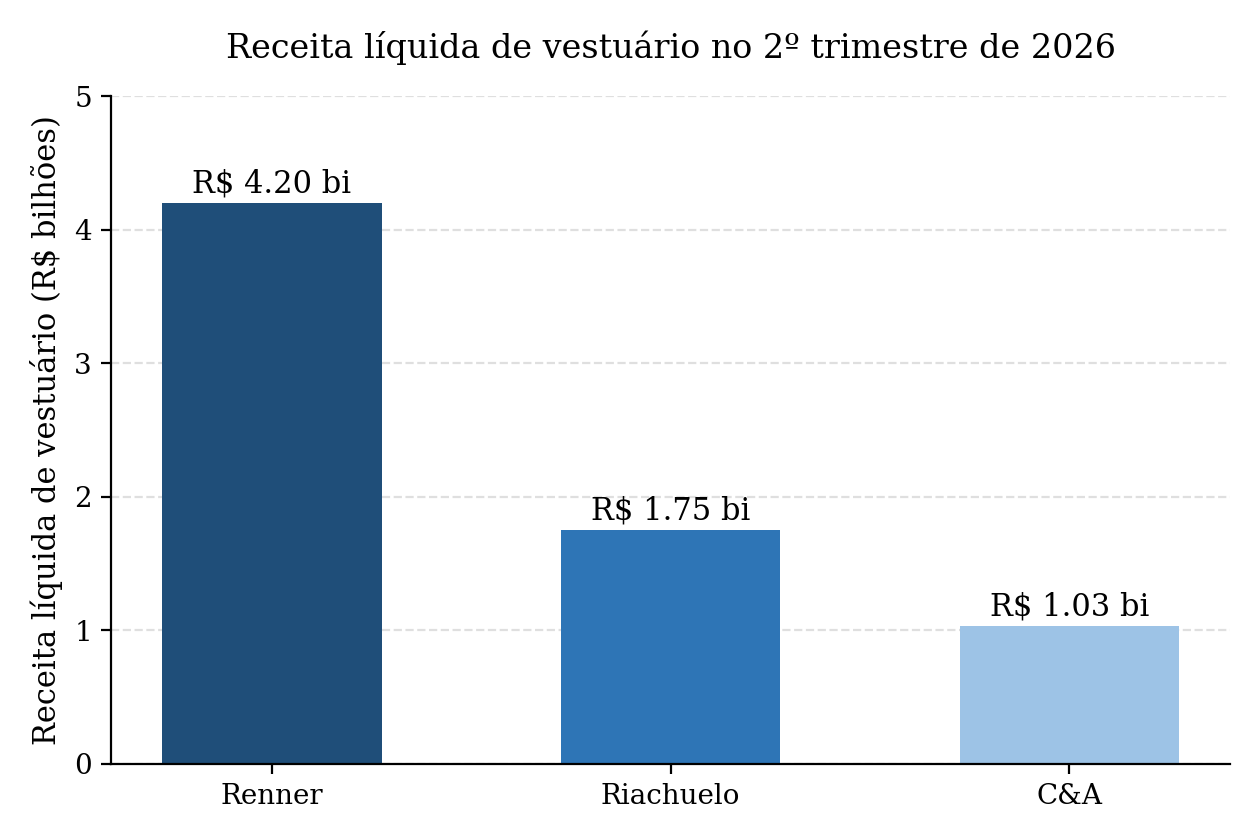
\includegraphics[width=0.75\textwidth]{imagens/mercado/receita_vestuario_2t2026.png}
    \source{Elaborado pelos autores (2026) com base em \citeonline{gbljeans2026trimestre}.}
\end{figure}

O SOM mais realista, no curto prazo, é a própria Riachuelo, cliente do projeto. A rede opera cerca de 440 lojas no Brasil \cite{exame2025riachuelo}, das quais apenas duas, a loja conceito de Curitiba e a do Shopping Eldorado, em Pinheiros, contam com self-checkout em todos os caixas, e a expansão prevista para 2026 abrange mais 15 a 20 lojas do mesmo formato \cite{promoview2026riachuelo}. Esse grupo de 15 a 20 lojas, e não a rede completa, representa o SOM do projeto, porque corresponde ao momento em que a companhia está padronizando a tecnologia de checkout que será replicada nas fases seguintes de expansão.

\begin{table}[htbp]
    \centering
    \caption{Estimativa de tamanho do mercado em três camadas}
    \label{tab:tam_sam_som}
    \footnotesize
    \renewcommand{\arraystretch}{1.35}
    \begin{tabularx}{\textwidth}{@{}
        >{\RaggedRight\arraybackslash}p{2.2cm}
        >{\RaggedRight\arraybackslash}X
        >{\RaggedRight\arraybackslash}p{3.6cm}
        >{\RaggedRight\arraybackslash}p{3.3cm}@{}}
        \toprule
        \textbf{Camada} & \textbf{Escopo} & \textbf{Tamanho estimado} & \textbf{Fonte} \\
        \midrule
        TAM (tecnológico) & Mercado global de RFID no varejo
            & US\$ 15,97 bi (2026) a US\$ 34,46 bi (2035)
            & \citeonline{businessresearch2026rfid} \\
        \addlinespace
        TAM (mercado-cliente) & Varejo têxtil brasileiro (vestuário, calçados, cama, mesa e banho)
            & R\$ 427,1 bi (2025)
            & \citeonline{gbljeans2026maiores}, dado ABVTEX \\
        \addlinespace
        SAM & Renner, Riachuelo e C\&A, redes com self-checkout implantado ou em piloto
            & R\$ 8,9 bi de receita líquida no trimestre; mais de R\$ 40 bi em vendas brutas anuais somadas
            & \citeonline{gbljeans2026trimestre}; \citeonline{gbljeans2026ranking} \\
        \addlinespace
        SOM & Riachuelo, onda de expansão de lojas conceito prevista para 2026
            & 15 a 20 lojas, de uma rede de cerca de 440
            & \citeonline{promoview2026riachuelo}; \citeonline{exame2025riachuelo} \\
        \bottomrule
    \end{tabularx}
    \source{Elaborado pelos autores (2026).}
\end{table}

\subsection{Síntese}
\label{subsec:sintese_mercado}

O panorama mostrou um varejo de moda de grande escala, mas concentrado em poucas redes de grande porte quando se trata de tecnologia de checkout avançada, e a equação de valor inteligente descrita pela Strategy\& reforçou por que a eficiência do checkout tende a ser prioridade mais natural no \textit{mass market} e no \textit{fast fashion} do que no premium ou no luxo. O segmento-alvo, formado pelas redes desse posicionamento com self-checkout implantado ou em piloto, corresponde a um SAM de cerca de R\$ 40 bilhões em vendas brutas anuais somadas entre Renner, Riachuelo e C\&A, dentro de um TAM tecnológico global de quase US\$ 16 bilhões. O SOM, as 15 a 20 lojas conceito que a Riachuelo prevê abrir em 2026, oferece um alvo comercial concreto e com prazo definido.
